%%%%%
\begin{figure}[!ht]
\centering
  \hfill\subfloat[]{
  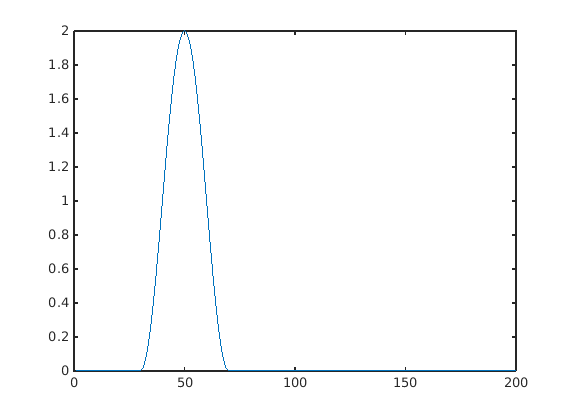
\includegraphics[width=0.35\textwidth]{t4i8_1}
  }\hfill
  \subfloat[]{%\label{fig:}
  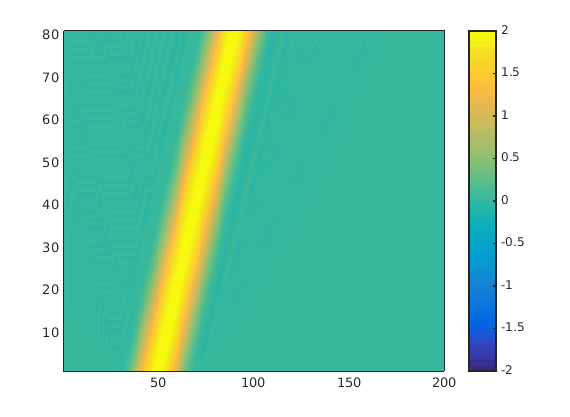
\includegraphics[width=0.35\textwidth]{t4i8_2}
  }\hfill
  \caption{a) condicion inicial y b) su evolución.}%
\label{fig:t4i8}
\end{figure}
%%%%%
